\subsection{View}

\begin{figure}[h]
	\centering
	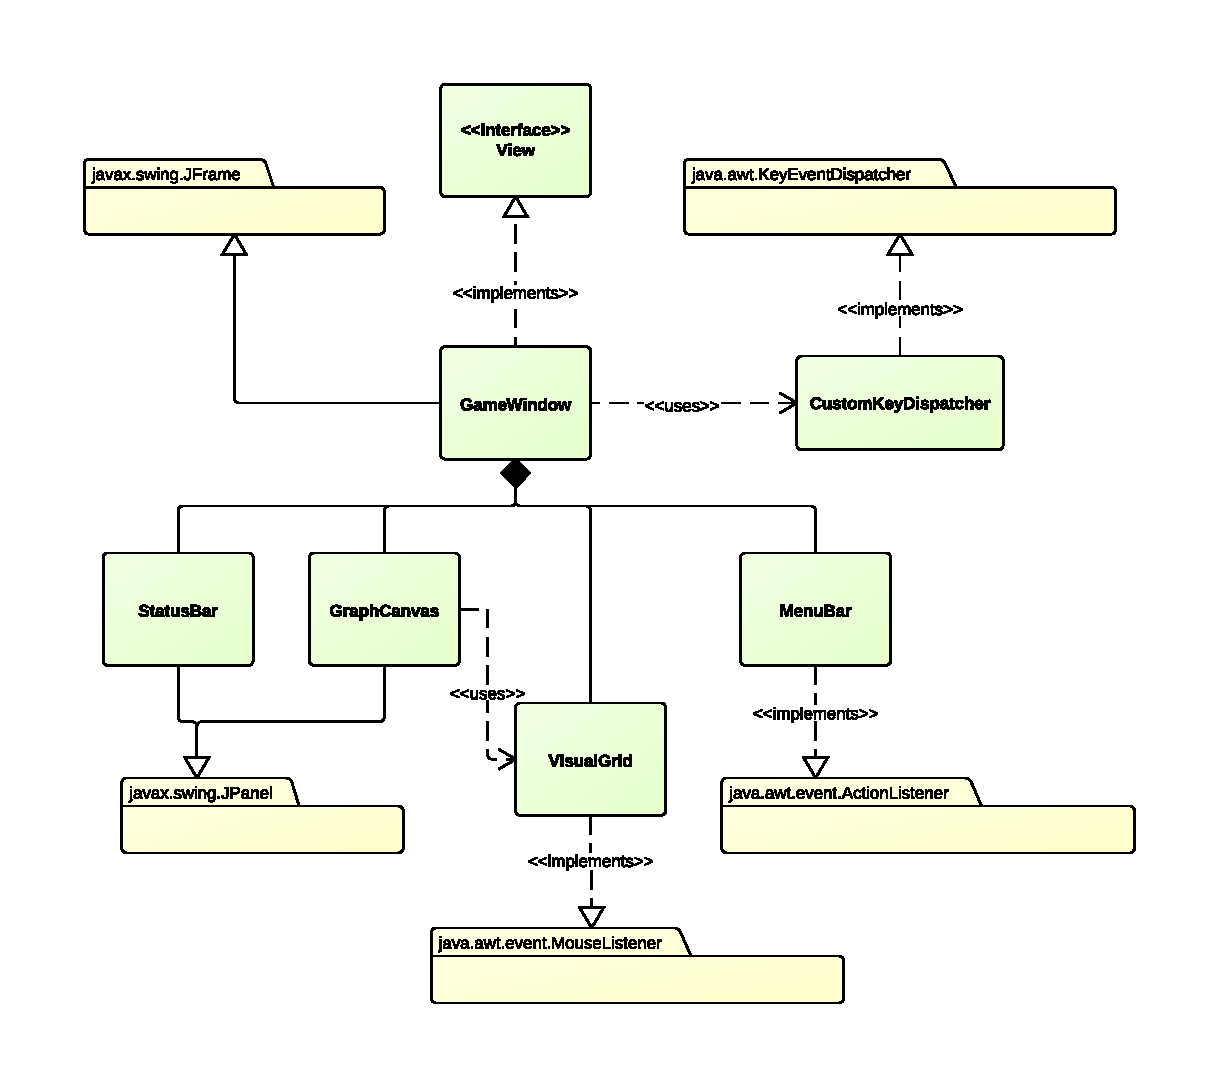
\includegraphics[page=1,width=\textwidth,keepaspectratio]{viewClassDiagram.pdf}
	\caption{View class diagram.}
	\label{img:viewClassDiagram}
\end{figure}
\pagebreak

% Interface View
\interface{View}{view}
View is an \gls{interface} for implementation of the \gls{gui}. \\ 

\centerdash

\paragraph*{Method Summary}
\paragraph*{}
\begin{longtable}{Lp{10cm}}
	\startmethodtable
	\method{public boolean}{registerController(ViewManager viewManager)}{view:registercontroller} \\
	& Registers a \ref{cls:viewmanager} as the controller for the user interface. \\
	\method{public boolean}{displayPopUp(String message)}{view:displaypopup} \\
	& Displays a message in a pop-up. \\
	\method{public boolean}{addCustomMenuItem(MenuItem item)}{view:addcustommenuitem} \\
	& Adds a custom \texttt{MenuItem} to the menu. \emph{facultative}\\ 
	\method{public boolean}{updatePlayerStatus(Player player)}{view:updateplayerstatus}\\
	& Updates the currently active \ref{cls:player} displayed. \\
	\method{public boolean}{displayErrorMessage(String message)}{view:displayerrormessage} \\
	& Displays a error message. \\
	\method{public boolean}{redrawGraph()}{view:redrawgraph} \\
	& Redraws the \ref{cls:graph}. \\ 
	\method{public boolean}{setVisualVertexSize(int size)}{view:setvisualvertexsize} \\
	& Sets the \texttt{size} of the \texttt{Vertices} displayed. \\ 
	\hline
\end{longtable}
\pagebreak

% GameWindow
\class{GameWindow}{gamewindow}
\createindentedlist{java.lang.Object, java.awt.Component, java.awt.Container, java.awt.Window, java.awt.Frame, javax.swing.JFrame, de.graphioli.view.GameWindow}

This class is the actual game window containing \ref{cls:graphcanvas}, \ref{cls:statusbar} and \ref{cls:menubar}. It handles keyboard inputs with a \ref{cls:customkeydispatcher}. \\ 
\interfaces{cls:view}

\centerdash

\paragraph*{Method Summary}
\paragraph*{}
\begin{longtable}{Lp{10cm}}
	\startmethodtable
	\method{public boolean}{registerController(ViewManager viewManager)}{view:registercontroller} \\
	& Registers a \ref{cls:viewmanager} as the controller of the GUI. \\
	\method{public boolean}{displayPopUp(String message)}{view:displaypopup} \\
	& Creates a pop-up to display a message. \\
	\method{public boolean}{addCustomMenuItem(MenuItem item)}{view:addcustommenuitem} \\
	& Adds a custom \texttt{MenuItem} to the menu in the \ref{cls:menubar}. \\ 
	\method{public boolean}{updatePlayerStatus(Player player)}{view:updateplayerstatus}\\
	& Updates the currently active \ref{cls:player} displayed in the \ref{cls:statusbar}. \\
	\method{public boolean}{displayErrorMessage(String message)}{view:displayerrormessage} \\
	& Displays an error message in the \ref{cls:statusbar}. \\
	\method{public boolean}{redrawGraph()}{view:redrawgraph} \\
	& Redraws the \ref{cls:graph} displayed in the \ref{cls:graphcanvas}. \\ 
	\method{public boolean}{setVisualVertexSize(int size)}{view:setvisualvertexsize} \\
	& Sets the \texttt{size} of the \texttt{Vertices} displayed. \\ 
	\method{public ViewManager}{getViewManager()}{gw:getviewmanager} \\
	& Returns the  associated \ref{cls:viewmanager}. \\
	\method{public boolean}{onKeyRelease(int keyCode)}{gw:onkeyrelease} \\
	& Forwards the key input to the \ref{cls:viewmanager}. \\
	\method{public File}{openFileDialog()}{gw:openfiledialog} \\
	& Opens a load file dialog. \\
	\method{public File}{saveFileDialog()}{gw:savefiledialog} \\
	& Opens a save file dialog. \\
	\hline
\end{longtable}
\pagebreak

% CustomKeyDispatcher
\class{CustomKeyDispatcher}{customkeydispatcher}
This class handles the keyboard input. \\ 

\begin{description}
	\item[All Implemented Interfaces] \hfill \\
	java.awt.KeyEventDispatcher
\end{description}

\centerdash

\paragraph*{Method Summary}
\paragraph*{}
\begin{longtable}{Lp{10cm}}
	\startmethodtable
	\method{public}{CustomKeyDispatcher(GameWindow gamewindow)}{ckd:customkeydispatcher} \\
	& Creates a \texttt{CustomKeyDispatcher} and registers its parent \ref{cls:gamewindow}. \\
	\method{public boolean}{dispatchKeyEvent(Keyevent event)}{ckd:dispatchkeyevent} \\
	& Dispatches the \texttt{KeyEvent} and calls the \ref{cls:gamewindow}. \\
	\hline
\end{longtable}
\pagebreak

% GraphCanvas
\class{GraphCanvas}{graphcanvas}
\createindentedlist{java.lang.Object, java.awt.Component, java.awt.Container, javax.swing.JComponent, javax.swing.JPanel, de.graphioli.view.GraphCanvas}

This class is responsible for displaying \ref{cls:graph} and \ref{cls:grid} and handles mouse clicks through a \ref{cls:visualgrid}. \\ 

\centerdash

\paragraph*{Method Summary}
\paragraph*{}
\begin{longtable}{Lp{10cm}}
	\startmethodtable
	\method{public}{GraphCanvas(GameWindow parent)}{gc:graphcanvas} \\
	& Creates a \texttt{GraphCanvas} and registers its parent \ref{cls:gamewindow}. \\
	\method{public boolean}{updateCanvas()}{gc:updatecanvas} \\
	& Updates and redraws the \texttt{GraphCanvas}. \\ 
	\hline
\end{longtable}
\pagebreak

% VisualGrid
\class{VisualGrid}{visualgrid}
This class handles mouse input, serves as an connector between \ref{cls:grid} and display and handles the size of the drawn \ref{cls:visualvertex}. \\ 
\begin{description}
	\item[All Implemented Interfaces] \hfill \\
	java.awt.event.MouseListener
\end{description}
\centerdash

\paragraph*{Method Summary}
\paragraph*{}
\begin{longtable}{Lp{10cm}}
	\startmethodtable
	\method{public}{VisualGrid(GameWindow parentGameWindow)}{vg:visualgrid} \\
	& Creates a \texttt{VisualGrid} and registers its parent \ref{cls:gamewindow}. \\
	\method{private GridPoint}{parseCoordinates(int xCoord, int yCoord)}{vs:parsecoordinates} \\
	& Parses the coordinates of the mouse click to the specific \ref{cls:gridpoint}. \\
	\method{public boolean}{setVisualVertexSize(int size)}{vs:setvisualvertexsize} \\
	& Sets the \texttt{size} of the displayed \texttt{Vertices} up to a \ref{cls:grid} specific maximum value. \\
	\method{public int}{getVisualVertexSize()}{vs:getvisualvertexsize} \\
	& Returns the \texttt{size} of the displayed \texttt{Vertices}. \\ 
	\method{public void}{mouseClicked(MouseEvent event)}{vs:mouseclicked} \\
	& Invoked if the mouse button has been clicked. \\ 
	\hline
\end{longtable}
\pagebreak

% MenuBar
\class{MenuBar}{menubar}
\createindentedlist{java.lang.Object, java.awt.Component, java.awt.Container, javax.swing.JComponent, javax.swing.JMenuBar, de.graphioli.view.MenuBar}

The \texttt{MenuBar} contains the game menu, options menu and help menu. It is displayed at the top of the \ref{cls:gamewindow} and starts the standard menu item specific methods. \\

\centerdash

\paragraph*{Method Summary}
\paragraph*{}
\begin{longtable}{Lp{10cm}}
	\startmethodtable
	\method{public}{MenuBar(GameWindow parent)}{mb:menubar} \\
	& Creates the \texttt{MenuBar} and registers its parent \ref{cls:gamewindow}. \\
	\method{private boolean}{createMenus()}{mb:addcustommenuitem} \\
	& Creates the standard menus including their menu items. \\ 
	\method{public boolean}{addCustomMenuItem(MenuItem item)}{mb:addcustommenuitem} \\
	& Adds a \texttt{MenuItem} to the options menu. \\ 
	\method{public void}{actionPerformed(ActionEvent event)}{mb:actionperformed} \\
	& Invoked when a \texttt{MenuItem} is selected. \\ 
	\hline
\end{longtable}
\pagebreak

% StatusBar
\class{StatusBar}{statusbar}
\createindentedlist{java.lang.Object, java.awt.Component, java.awt.Container, javax.swing.JComponent, javax.swing.JPanel, de.graphioli.view.StatusBar}

The \texttt{StatusBar} displays the currently active \ref{cls:player} and a short status or error message. \\

\centerdash

\paragraph*{Method Summary}
\paragraph*{}
\begin{longtable}{Lp{10cm}}
	\startmethodtable
	\method{public boolean}{updatePlayerStatus(Player player)}{sb:updateplayerstatus} \\
	& Updates the currently active \ref{cls:player} displayed. \\ 
	\method{public boolean}{displayedErrorMessage(String message)}{sb:displayerrormessage} \\
	& Displays a status or error message. \\ 
	\hline
\end{longtable}
